%=======================+=========================
%==============  DAQ   ================
%=================================================\

\section[Data Acquisition]{Data acquisition \label{sec:daq}}

%\subsection{Architecture \label{sec:daqarchitecture}}

%\subsection{Performance \label{sec:daqperformance}}

The \gx{} data acquisition software uses the CEBAF Online Data Acquisition (CODA) framework. CODA is a software toolkit of applications and libraries that allows customized data acquisition systems based on distributed commercial networks. A detailed description of CODA software and hardware can be found in Ref.\,\cite{CLAS12DAQ}. 

The maximum readout capability of the electronics in the VME/VXS crate is 200 MB/s per crate and the number of crates producing data is about 55.
The data from the electronic modules are read via the VME back-plane (2eSST, parallel bus) by the crate readout controller (ROC), which is a single-board computer running Linux.
The \gx~ network layout and data flow are shown in Fig.~\ref{fig:CODA}.
Typical data rates from a single ROC are in the range of 20--70~MB/s, depending on the detector type and trigger rate.
The ROC transfers data over 1~Gbit Ethernet links to Data Concentrators (DC) using buffers containing event fragments from 40 triggers at a time. Data Concentrators are programs that build partial events received from 10-12 crates and run on a dedicated computer node.
The DC output traffic of 200-600 MB/s is routed to the Event Builder (EB) to build complete events.
The Event Recorder (ER), which is typically running on the same node as an Event Builder, writes data to local data storage.
\gx{} has been collecting data at a rate of 500--900 MB/s, which allows the ER to write out to a single output stream. The system is expandable to handle higher luminosity where rates rise to 1.5--2.5~GB/s. In this case, the ER must write multi-stream data to several files in parallel.
All DAQ computer nodes are connected to both a 40 Gb Ethernet switch and a 56 Gb Infiniband switch.
The Ethernet network is used exclusively for DAQ purposes: receiving data from detectors, building events, and writing data to disk, 
while the Infiniband network is used to transfer events for online data quality monitoring. 
This allows decoupling DAQ and monitoring network traffic.
The livetime of the DAQ is in the range of 92--100\%. The deadtime arises from readout electronics and depends on the trigger rate.  
The DAQ software does not cause dead time during an experimental run, but software-related dead time appears while stopping and starting the run, which takes between 2-8 minutes. 

\begin{figure}[tbp]
\begin{center}
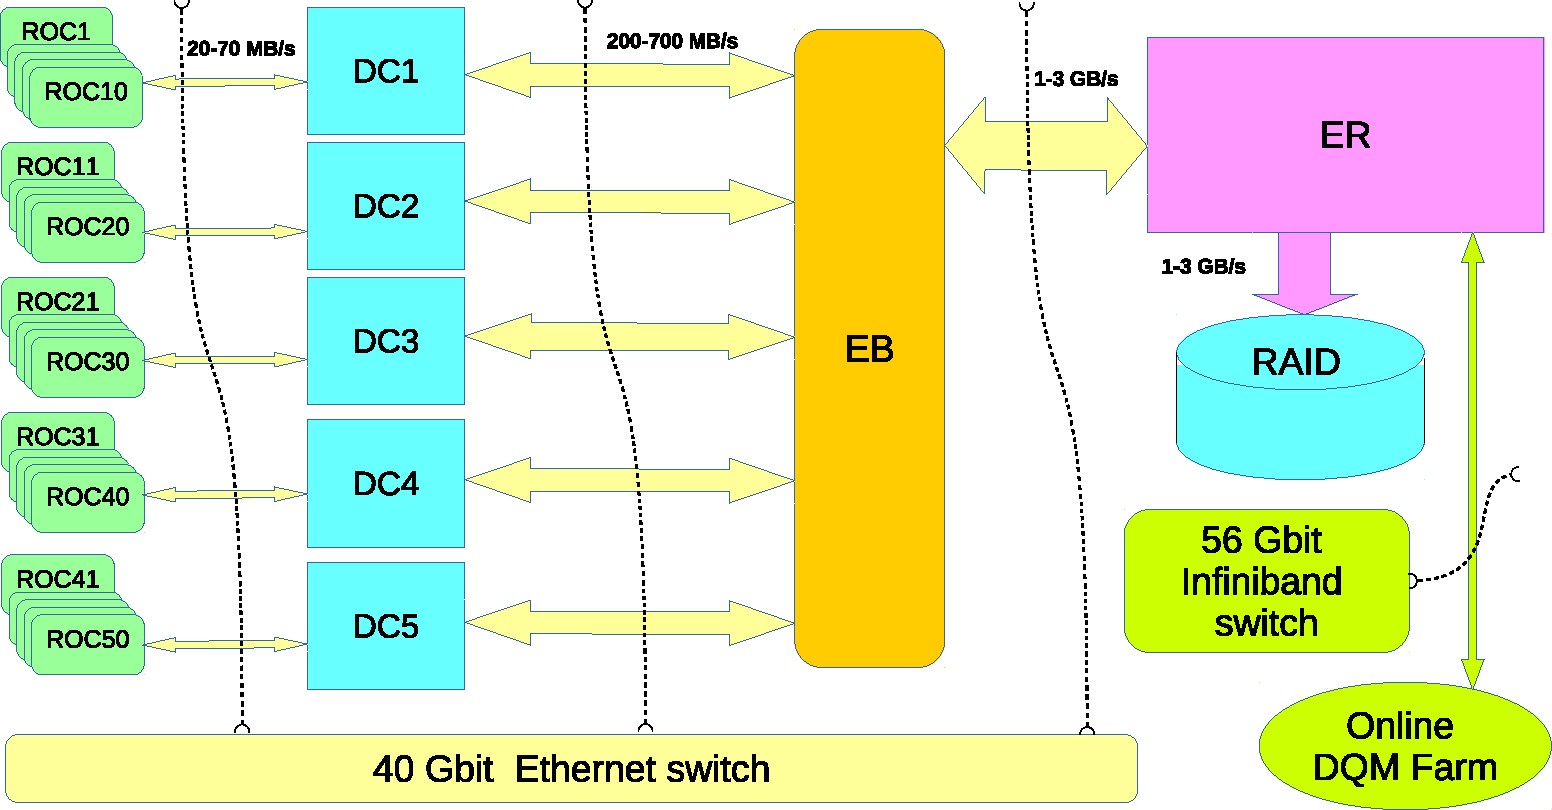
\includegraphics[width=0.75\textwidth]{figures/DAQ_coda.pdf}  
\caption{ \label{fig:CODA}
Schematic DAQ configuration for \gx. The high-speed DAQ connections between the ROCs and the ER are contained within an isolated network. The logical data paths are indicated by arrows,
although physically they are routed through the 40 Gbit ethernet switch.  The online monitoring system uses its own separate 56 Infiniband switch.}

\end{center}
\end{figure}
